% !TeX program = xelatex 
\documentclass{hitreport}
\usepackage{url}
\usepackage{algorithm,float}  
\usepackage{algpseudocode}  
\usepackage{amsmath}
\usepackage{cite}
\usepackage{threeparttable}
\usepackage{subfig}
\usepackage{listings} %插入代码
\usepackage{xcolor} %代码高亮
\usepackage{tikz}
\usepackage{hyperref}
\usepackage{wasysym}
\usepackage{pgfplots}
\usetikzlibrary{positioning}




\lstset{numbers=left, %设置行号位置
	numberstyle=\tiny, %设置行号大小
	keywordstyle=\color{blue}, %设置关键字颜色
	commentstyle=\color[cmyk]{1,0,1,0}, %设置注释颜色
	frame=single, %设置边框格式
	escapeinside=``, %逃逸字符(1左面的键),用于显示中文
	breaklines, %自动折行
	extendedchars=false, %解决代码跨页时,章节标题,页眉等汉字不显示的问题
	xleftmargin=2em,xrightmargin=2em, aboveskip=1em, %设置边距
	tabsize=4, %设置tab空格数
	showspaces=false %不显示空格
}

\renewcommand{\algorithmicrequire}{\textbf{Input:}}  % Use Input in the format of Algorithm  
\renewcommand{\algorithmicensure}{\textbf{Output:}} % Use Output in the format of Algorithm  

\makeatletter
\newenvironment{breakablealgorithm}
  {% \begin{breakablealgorithm}
   \begin{center}
     \refstepcounter{algorithm}% New algorithm
     \hrule height.8pt depth0pt \kern2pt% \@fs@pre for \@fs@ruled
     \renewcommand{\caption}[2][\relax]{% Make a new \caption
       {\raggedright\textbf{\ALG@name~\thealgorithm} ##2\par}%
       \ifx\relax##1\relax % #1 is \relax
         \addcontentsline{loa}{algorithm}{\protect\numberline{\thealgorithm}##2}%
       \else % #1 is not \relax
         \addcontentsline{loa}{algorithm}{\protect\numberline{\thealgorithm}##1}%
       \fi
       \kern2pt\hrule\kern2pt
     }
  }{% \end{breakablealgorithm}
     \kern2pt\hrule\relax% \@fs@post for \@fs@ruled
   \end{center}
  }
\makeatother

% =============================================
% Part 0 Edit the info
% =============================================

\major{计算机科学与技术}
\name{孙骁}
\title{视听觉信号处理\\实验报告}
\stuid{1180300811} % 学号
\college{计算学部}
\date{2020年12月23日}
\lab{格物207} %实验地点
\course{视听觉信号处理}
\instructor{郑铁然}
% \grades{}
\expname{DPCM编解码实验} %实验名称
% \exptype{} % 实验类型
% \partner{} % 同组学生名字
\term{2020秋季学期}

\begin{document}

\maketitle

\tableofcontents
\newpage
% =============================================
% Part 1 Header
% =============================================



% =============================================
% Part 2 Main document
% =============================================

\section{实验内容与步骤}

\subsection{DPCM编解码算法}

\subsubsection{编码算法}

\begin{enumerate}
\item 从wav文件中读入原始数据;
\item 与解码后的$\bar{x}\left( n - 1 \right) $计算差值;
\item 对从$d\left(n\right)$进行重新量化,要求8bit,一个采样一个BYTE;

直接量化或量化因子法(推荐);

\item 解码;
\item 对从$d\left(n\right)$进行重新量化,要求4bit,两个采样一个BYTE;

\begin{enumerate}
\item 直接量化;
\item 设计一个因子a;
\item 对数变换。
\end{enumerate}

\item 解码计算$\bar{x}\left(n-1\right)$
\begin{enumerate}
\item 量化因子法:$\bar{x}\left(n\right) = \bar{x}\left(n-1\right) + \left(c\left(n\right) - 8\right) \times a$;
\item 对数变换法:$\bar{x}\left(n\right) = \bar{x}\left(n-1\right) + \left(-1\right)^{\text{sgn}\left(c\left(n\right) - 8\right)} \times a^{c\left(n\right) \& 7}$
\end{enumerate}

\item 封装$c\left(n\right)$;
\item 保存编码到文件(后缀用”.dpc”)。

\end{enumerate}

\subsubsection{解码算法}

解码还原后文件,保存为pcm文件。

\subsection{改进思路}

请提出你的若干改进策略(可聚焦于8bit量化编码进行改进)。

\subsection{计算信噪比}



\section{实验环境}

\begin{enumerate}
\item Anaconda 4.8.4
\item Python 3.7.4
\item PyCharm 2020.3 (Professional Edition)
\item Windows 10 2004
\end{enumerate}

\section{实验原理}

\subsection{DPCM编解码算法}\label{sec:energy}

由于相邻采样值之间的差值远小于采样值本身,可以对差值进行编码,而不是对采样值本身进行编码,这就是差分脉冲编码DPCM。

产生差分信号的过程:直接存储前一次的采样值,用本次的采样值计算差值,经过量化得到数字语音编码。解码端做相反处理,恢复原信号。用Z变换考查各点信号的时域关系,有
\begin{align}
C\left(z\right) = X\left(z\right)\left(1-z^{-1}\right) +E\left(z\right)
\end{align}
和
\begin{align}
\bar{X}\left(z\right) = \frac{C\left(z\right)}{1-z^{-1}} = X\left(z\right) + \frac{E\left(z\right)}{1-z^{-1}}.
\end{align}
式中,$E\left(z\right)$为量化器量化噪声$e\left(n\right)$的Z变换。

由于量化器的量化噪声被累积叠加到了输出信号中,即每次的量化噪声信号都被保存,叠加到下次的输出当中,如果量化噪声始终是同一方向,则输出信号会越来越偏离原信号。因此,编码器应采用前一次解码后的采样值代替前一次的输入采样值,以生成差分信号。

则
\begin{align}
\widetilde{X}\left(z\right) = \frac{C\left(z\right)z^{-1}}{1-z^{-1}}.
\end{align}
编码结果为
\begin{align}
C\left(z\right) = X\left(z\right) - \widetilde{X}\left(z\right)+E\left(z\right),
\end{align}
代入后有
\begin{align}
C\left(z\right) = \left(X\left(z\right)+E\left(z\right)\right)\left(1-z^{-1}\right).
\end{align}
因此有
\begin{align}
\bar{X}\left(z\right) = \frac{C\left(z\right)}{1-z^{-1}} = X\left(z\right) + E\left(z\right),
\end{align}
由此可见,已经消除了量化噪声的累积。

DPCM仅仅用到了两个采样值之间的相关性。然而,当前输入采样不仅与上一时刻的采样值相关,也与前面若干采样值相关,可以使用线性预测分析的方法实现一般形式的差分脉冲编码。根据线性预测分析的原理,可以用过去的一些采样值的线性组合来预测和推断当前的采样值,得到一组线性预测系数,且预测误差$e\left(n\right)$的动态范围和平均能量均比信号$x\left(n\right)$小得多,预测阶数越高,预测误差越小,相应的编码速率可以越低。


\section{实验步骤及相应结果}

此部分内容与word模板相应章节对应,单击图片引用序号可以跳转查看相应图片结果。

\subsection{ 8bits DPCM编解码算法}

当量化因子取1时,量化因子法即为直接量化法,故在算法介绍时不分开介绍,在计算信噪比时做区分。

\subsubsection{简述算法内容}\label{sec:the}

8bit的编码算法,要求对$d\left(n\right)$重新量化,一个采样一个Byte。8位能表示的无符号数的范围是$\left(-128, 127\right)$,编码时采用取自然对数变换压缩编码,因此8位编码可表示的范围远大于信号的范围。

编码方法为,如果采样值为正数,则取自然对数的绝对值,转化为无符号int类型,保存为无符号int类型;如果采样值为负数,则取自然对数的绝对值,转化为无符号int类型,用255减去这个数,保存相减的数值。解码时,如果待解码数据范围为$\left[0,127\right)$,说明在编码前原数据是正数,直接做幂运算即可;如果待解码数据范围为$\left[128, 255\right)$,说明在编码前原数据为负数,先用255减去待解码数据,再做幂运算。

编码的过程中,为了避免量化噪声叠加到输出信号中,采用边编码边解码的方法,即采用前一次解码后的采样值代替前一次的输入采样值生成差分信号。在编码过程中维护两个列表,code\_data保存编码后的数据,decode\_data保存解码的数据,以备下一位编码使用。

写入dpc文件时,按照二进制格式打开,直接将编码后的8 bit无符号数写入即可。从dpc文件读出解码时,以二进制的形式读取文件,每次读取一个字节,调用struct.unpack函数,按照unsigned char解码得到对应的十进制数,直接解码第一个数;对于其他数据,将解码后与前一个解压缩的数据相加即得到本位的解压数据。

重新写回pcm文件时,需要为pcm文件配置声道数,量化位数和采样频率,将解码得到的列表转化为二进制数据写入.pcm 文件中。

按照公式(\ref{equ:snr})计算信噪比。
\begin{align}\label{equ:snr}
\text{SNR} = 10\times \log_{10}\frac{\sum_{n=0}^{M}x^2\left(n\right)}{\sum_{n=0}^{M}\left(\bar{x}\left(n\right) - x\left(n\right)\right)^2}
\end{align}

\subsubsection{解码信号的信噪比}

8bit DPCM编码算法使用直接量化法的信噪比为15.225,采用量化因子为23的量化因子算法的信噪比为13.199。

直接量化法解码后的波形如图(\ref{fig:81})所示,量化因子算法解码后的波形如图(\ref{fig:8q})所示。

\begin{figure}[htb]
	\centering
	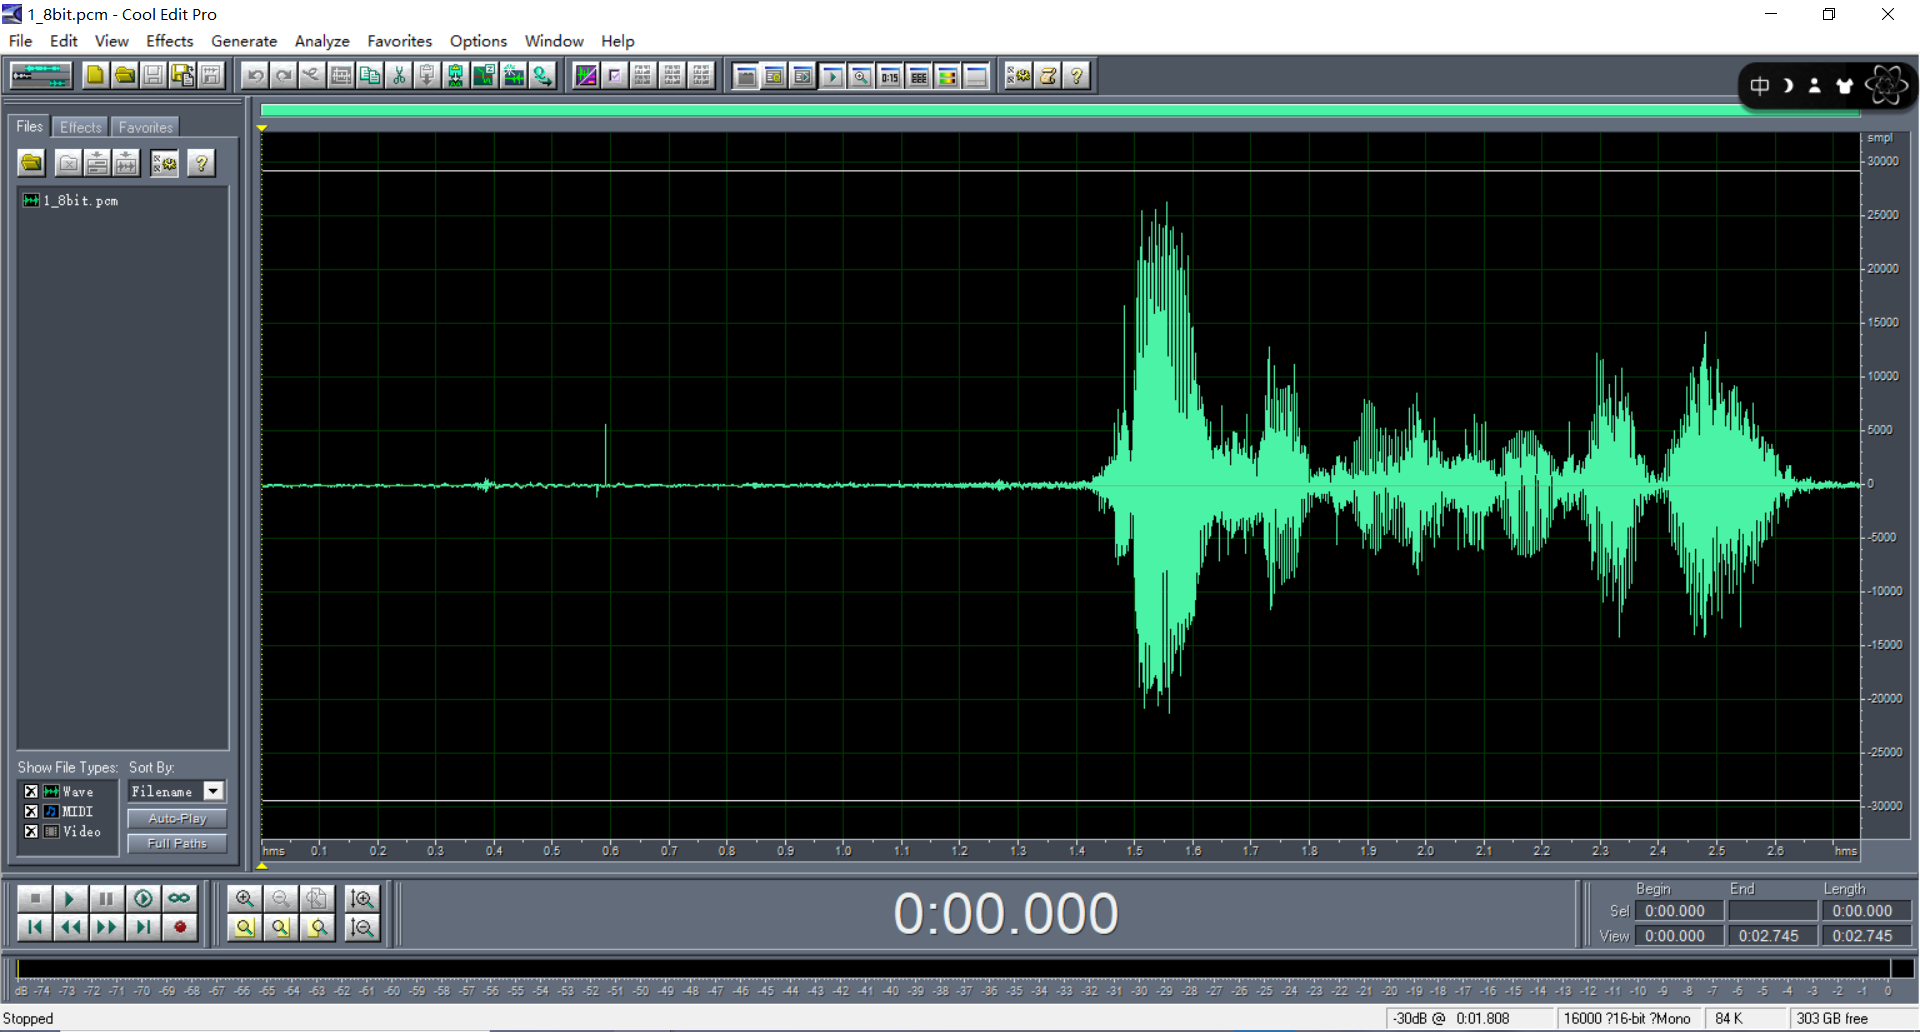
\includegraphics[width=0.9\linewidth]{81.png}
	\caption{8 bits DPCM编码直接量化法解码波形}\label{fig:81}
\end{figure}

\begin{figure}[htb]
	\centering
	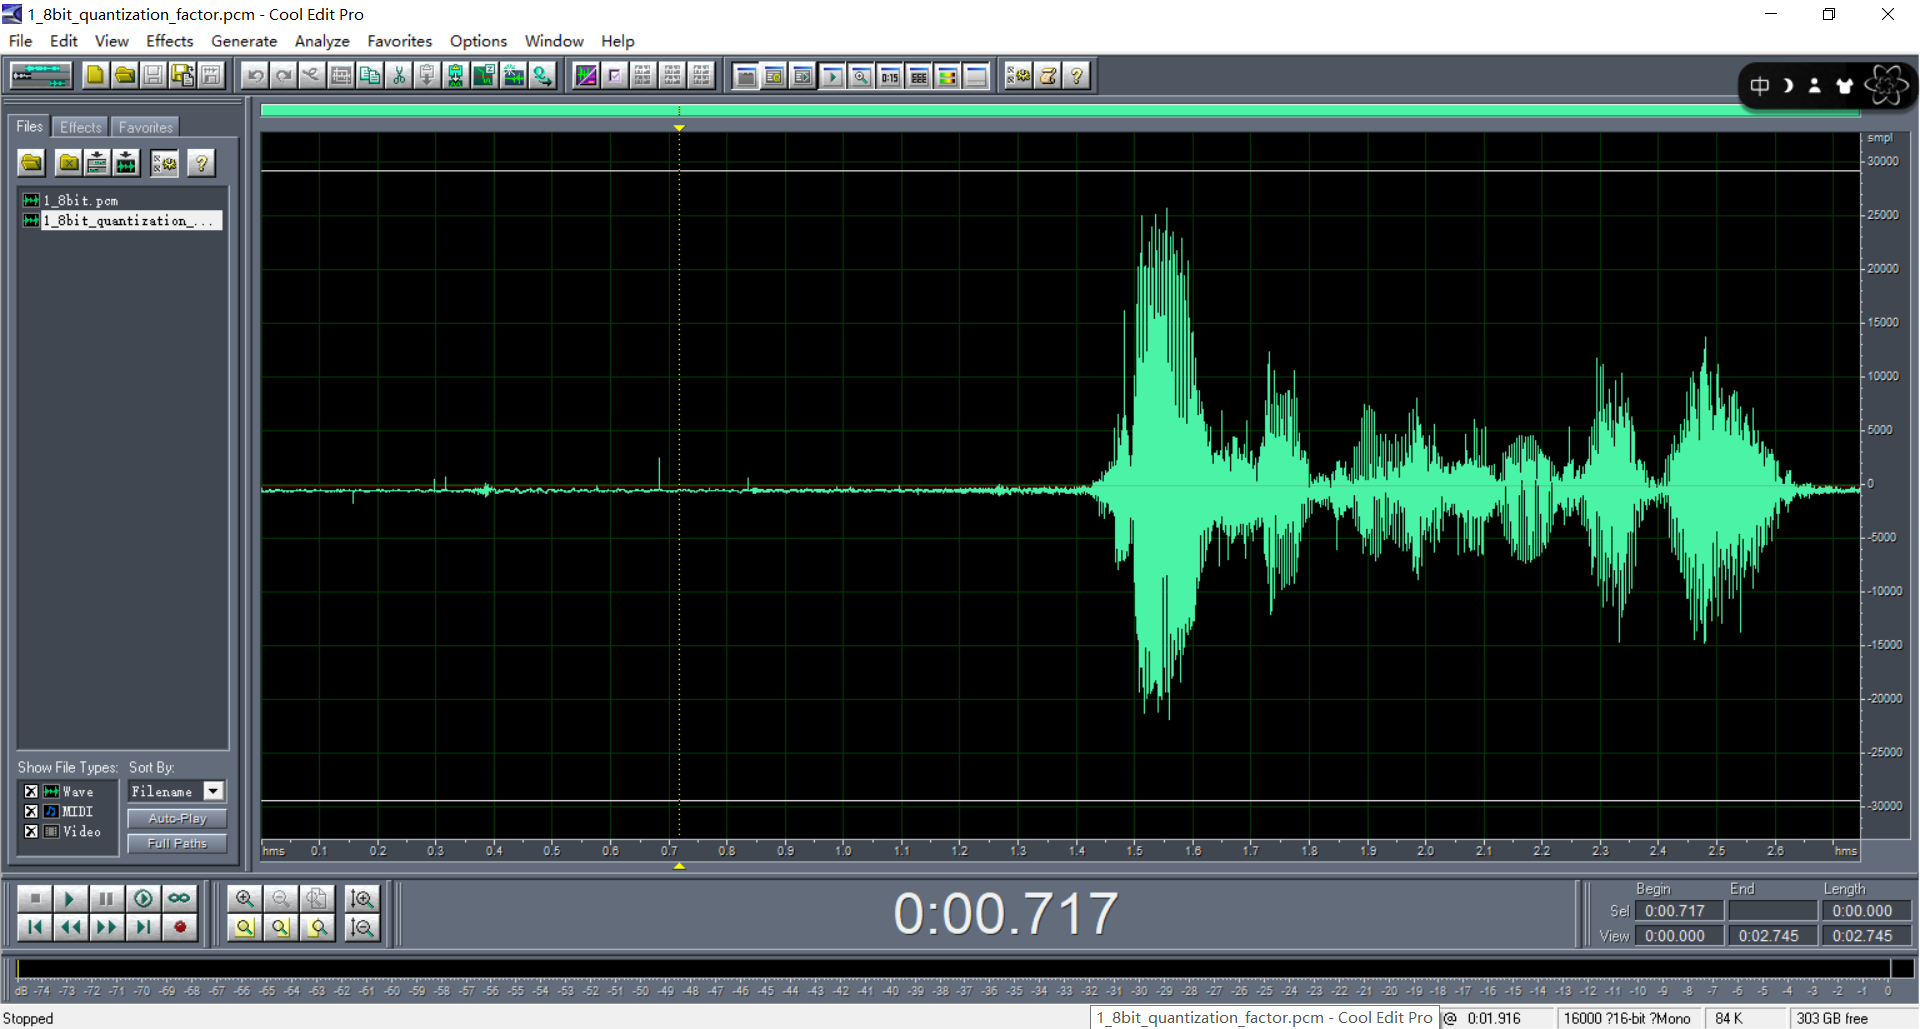
\includegraphics[width=0.9\linewidth]{8q.png}
	\caption{8 bits DPCM编码量化因子法解码波形}\label{fig:8q}
\end{figure}


\subsection{ 4bits DPCM编解码算法}\label{sec:sec2}

\subsubsection{你所采用的量化因子}

量化因子为23.

\subsubsection{拷贝你的算法,加上适当的注释说明}

\begin{lstlisting}[language=python]
def difference_pulse_coding_modulation_4(self):
	"""
	4 bits 编码的主函数
	"""
    print('DPCM 4bits')
    for key in self.wav_dic.keys():
        code_data = np.zeros_like(self.wav_dic[key][4]) # 编码的数据
        decode_data = np.zeros_like(self.wav_dic[key][4]) # 边编码边解码保存的临时数据
        length = len(self.wav_dic[key][4])
        code_data[0], decode_data[0] = self.coding_first_4(self.wav_dic[key][4][0]) # 对第一位特殊处理,计算编码和解码数据
        for i in range(1, length):
            err = self.wav_dic[key][4][i] - decode_data[i - 1]
            code_data[i] = self.dpcm_4(err) # 计算编码数据
            decode_data[i] = decode_data[i - 1] - self.__quantization_factor * np.exp(
                15 - code_data[i]) if err < 0 else decode_data[i - 1] + self.__quantization_factor * np.exp(
                code_data[i]) # 计算解码数据
        self.code_dic_4[key] = code_data # 将对应的文件存储到相应键值中
        # print(code_data)

def coding_first_4(self, data):
    """
    对第一位数据进行4 bits编码
    :param data: 第一位数据
    :return: 第一位数据编码结果与解码结果
    """
    if data < 0:
        code_data = 15 if data > -self.__quantization_factor else 15 - (
                np.uint8(int(abs(np.log(-data / self.__quantization_factor)) + 0.5) << 4) >> 4) # 若采样值小于零
        code_data = max(8, code_data)
        return code_data, np.exp(15 - code_data) * -self.__quantization_factor
    else:
        code_data = 0 if data < self.__quantization_factor else np.uint8(
            int(abs(np.log(data / self.__quantization_factor)) + 0.5) << 4) >> 4 # 若采样值大于零
        code_data = min(7, code_data)
        return code_data, np.exp(code_data) * self.__quantization_factor


def dpcm_4(self, data):
    """
    对其他数据进行4 bits编码
    :param data: 相应采样数据
    :return: 采样编码结果与解码结果
    """
    if data < 0:
        code_data = 15 if data > -self.__quantization_factor else 15 - (
                np.uint8(int(abs(np.log(-data / self.__quantization_factor)) + 0.5) << 4) >> 4) # 若采样值小于零
        code_data = max(8, code_data)
        # print(code_data)
        return code_data
    else:
        code_data = 0 if data < self.__quantization_factor else np.uint8(
            int(abs(np.log(data / self.__quantization_factor)) + 0.5) << 4) >> 4 # 若采样值大于零
        code_data = min(7, code_data)
        # print(code_data)
        return code_data
\end{lstlisting}

\subsubsection{解码信号的信噪比}

采用直接量化法的信噪比为3.948,采用量化因子法的信噪比为15.606。

直接量化法解码后的波形如图(\ref{fig:41})所示,量化因子算法解码后的波形如图(\ref{fig:4q})所示。

\begin{figure}[htb]
	\centering
	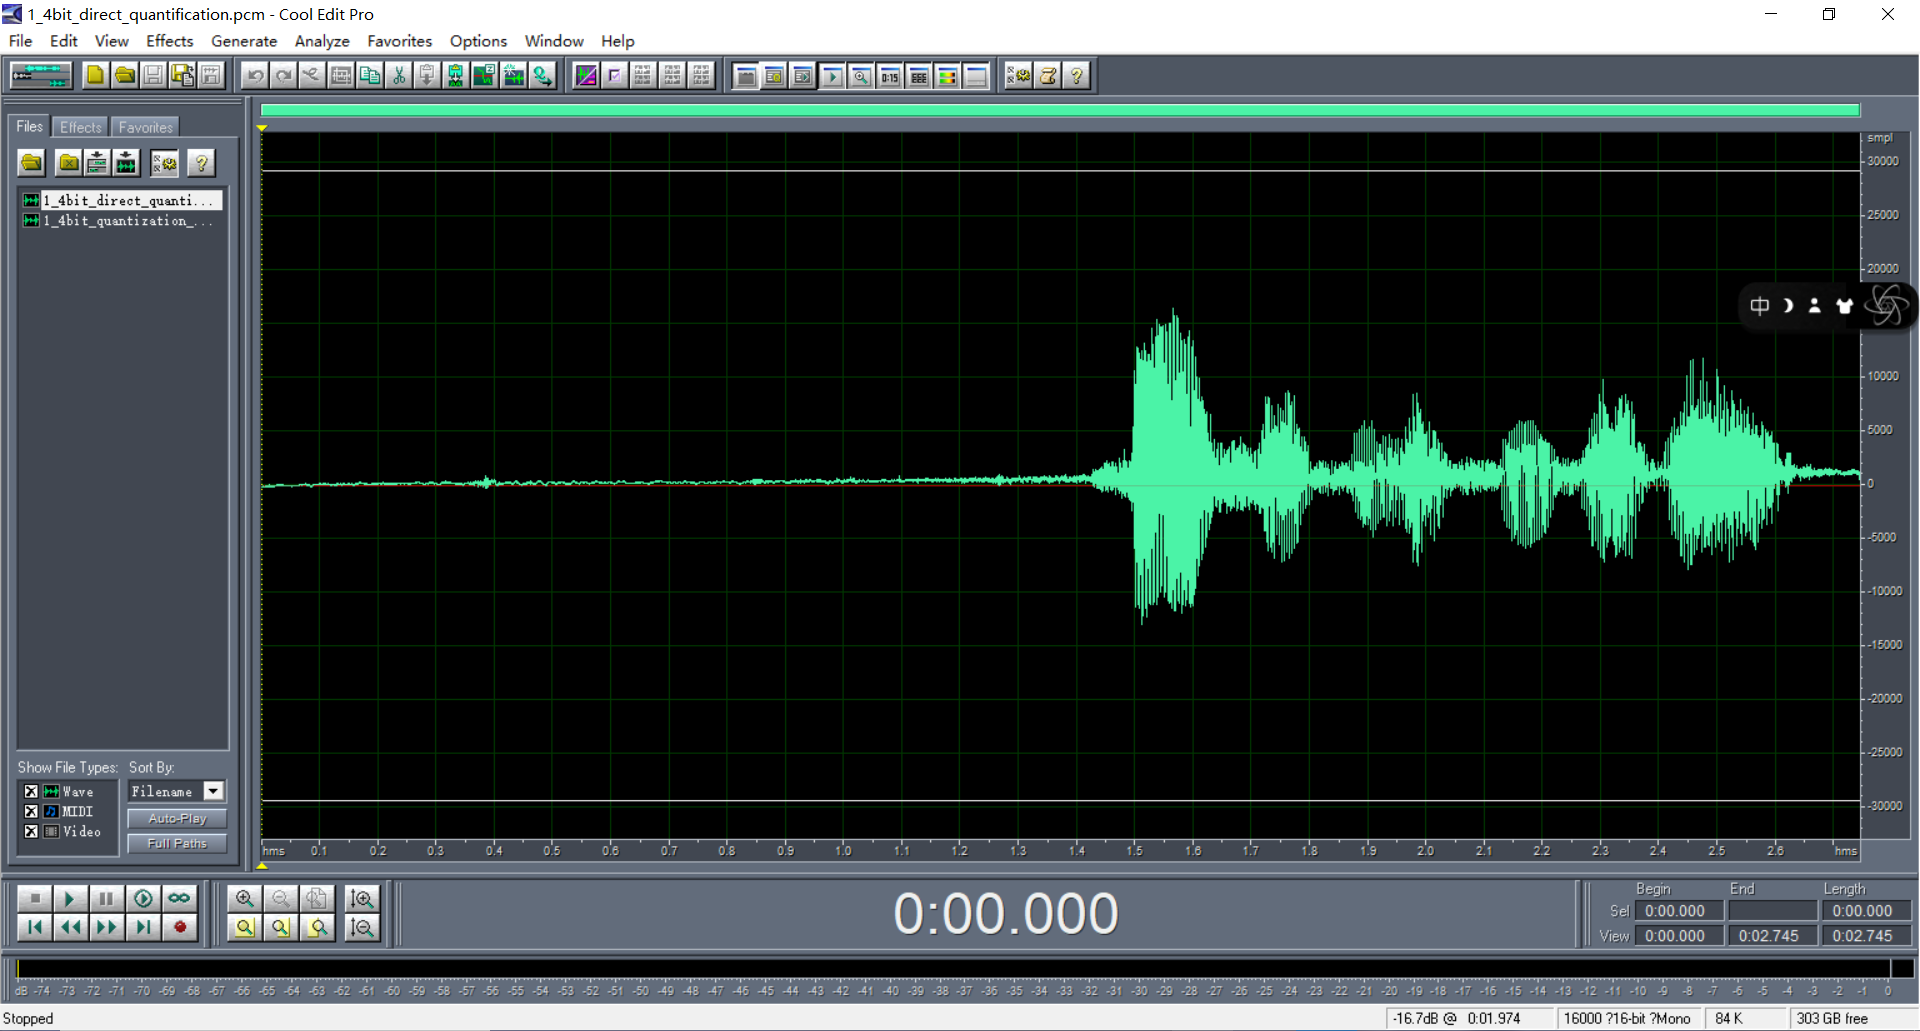
\includegraphics[width=0.9\linewidth]{41.png}
	\caption{4 bits DPCM编码直接量化法解码波形}\label{fig:41}
\end{figure}

\begin{figure}[htb]
	\centering
	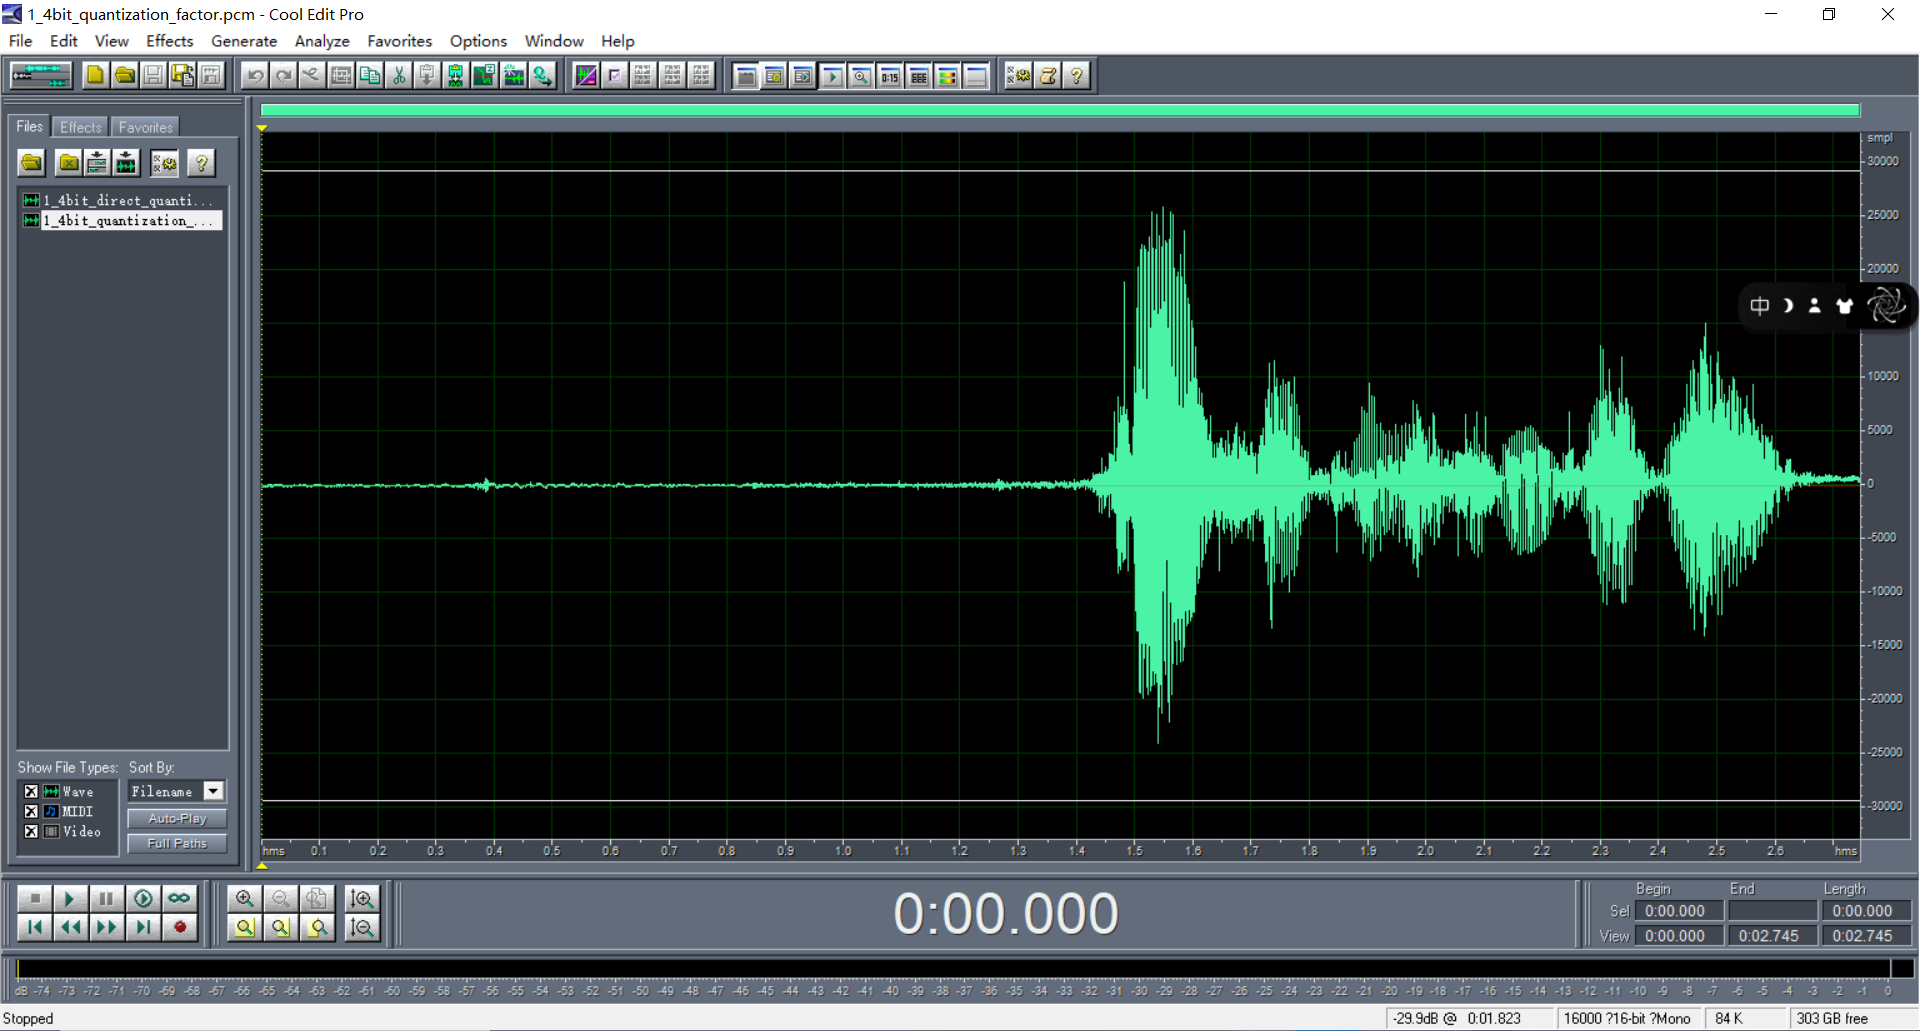
\includegraphics[width=0.9\linewidth]{4q.png}
	\caption{4 bits DPCM编码量化因子法解码波形}\label{fig:4q}
\end{figure}


\subsection{改进策略}\label{sec:sec3}

\subsubsection{对采样值做对数变换}

在章节\ref{sec:the}中,提到将原数据先取自然对数的绝对值再做编码,实际上最开始的实现是直接将原数据与编码后数据作差得到新的数据,但是在实际过程中发现舍入误差过大,因此转为先取对数在计算差分,取对运算为严格的单调递增变换,所以不影响数据的变化趋势,好处是用较小的值表示了较大范围的数据。

修改后的编码和解码方式为
\begin{align}
\begin{split}
d\left(n\right) = \log x\left(n\right) - \log \bar{x}\left(n\right)\\
\bar{x}\left(n\right) = \bar{x}\left(n-1\right) + x\left(n\right)\times a
\end{split}
\end{align}
其中,\textit{a}为量化因子,针对采样值为正数和负数的不同情况还要做不同处理。

采用量化因子编码,8 bit编码修改前的信噪比为5.432,修改后的信噪比为13.199。

\subsubsection{将小于量化因子的采样编码为固定值}

在8 bits 编码时,将绝对值小于量化因子的采样值直接编码为0,这样可以使很多较小采样值的编码一致,在语音恢复后,也不会有较大的影响,同样也提高了信噪比。

\subsubsection{可能的优化方向}

如果有更多的时间,我会做更一般的DCPM算法,因为实验中实现DPCM仅仅用到了两个采样值之间的相关性。然而,当前输入采样不仅与上一时刻的采样值相关,也与前面若干采样值相关,可以使用线性预测分析的方法实现更一般形式的差分脉冲编码。根据线性预测分析的原理,可以用过去的一些采样值的线性组合来预测和推断当前的采样值,得到一组线性预测系数,且预测误差$e\left(n\right)$的动态范围和平均能量均比信号$x\left(n\right)$小得多,预测阶数越高,预测误差越小,相应的编码速率可以越低。

\subsection{简述你对量化误差的理解}

\subsubsection{什么是量化误差}

一般量化值都用二进制表示,如果用m个二进制数表示量化值,即量化字长,那么一般将幅度值划分为 $2^m$ 个等分区间。
从量化的过程中可以看出,信号在经过量化后,一定存在一个量化误差。其定
义为
\begin{align}
e\left(n\right) = \bar{x}\left(n\right) - x\left(n\right)
\end{align}
式中,$e\left(n\right)$为量化误差或者噪声,$\bar{x}\left(n\right)$为量化后的采样值,即量化器的输出,$x\left(n\right)$为未量化的采样值,即量化器的输入。

此外,在信号压缩存储的过程中,也会产生量化误差。


\subsubsection{为什会编码器中会有一个解码器}

在章节\ref{sec:energy}的DPCM算法介绍中,已经对此部分做了解释。简言之,如果对编码信号做差分计算,会导致每次编码的量化误差都被保存下来,如果量化噪声始终是同一方向,则输出信号会越来越偏离原信号。因此,编码器应采用前一次解码后的采样值代替前一次的输入采样值,以生成差分信号。

\section{总结}

\subsection{请总结本次实验的收获}

对DPCM编解码算法有了新的认识,对于不同的量化方法有了深刻的了解。

\subsection{请给出对本次实验内容的建议}

无。

 
\renewcommand\refname{参考文献}
 
\bibliographystyle{unsrt} %%参考文献的格式(可选的格式还有:plain)
 
\bibliography{Refer.bib}    %%参考文件存储位置

\newpage
\begin{appendices}

\section{从wav文件读取数据——read\_wav\_from\_file.py}

\lstinputlisting[language=python]{code/read_wav_from_file.py}

\section{计算信噪比——calculate\_snr.py}

\lstinputlisting[language=python]{code/calculate_snr.py}

\section{编码核心代码——code\_wav\_file.py}

\lstinputlisting[language=python]{code/code_wav_file.py}

\section{解码过程读取编码后的文件——read\_dpc\_from\_file.py}

\lstinputlisting[language=python]{code/read_dpc_from_file.py}

\section{将编码后的结果写入文件——write\_dpc\_to\_file.py}

\lstinputlisting[language=python]{code/write_dpc_to_file.py}

\end{appendices}

\end{document}
